\documentclass[prd,aps,twocolumn,a4paper,showkeys,nofootinbib]{revtex4-2}

\usepackage{amsmath}
\usepackage{amsfonts}
\usepackage{amssymb}	
\usepackage{graphicx}
\usepackage{color}
\usepackage[hidelinks]{hyperref}
\allowdisplaybreaks

\def\TODO{\textcolor{red}{TODO:}}
\def\Mc{{\cal M}_c}

\begin{document}

\title{Classification of NS data}

\author{Marina Berbel, Miquel Miravet-Tenés}

\date{\today}

\maketitle

%==========================================================
\section{Random forest}
%==========================================================


\subsection{Using only independent recovered variables}
Training and testing using: $m1_{rec}, m2_{rec}, chi1_{rec}, chi2_{rec}, snr$.
Standard deviation of score during crossvalidation:  0.000277942225285724 . Mean:  0.9744487408123469
Score  0.9748495808263471 . Optimum forest found:  200  trees,  entropy  criteria and  sqrt  max features

Score on testing:  0.9747829130485508

\begin{figure}[]
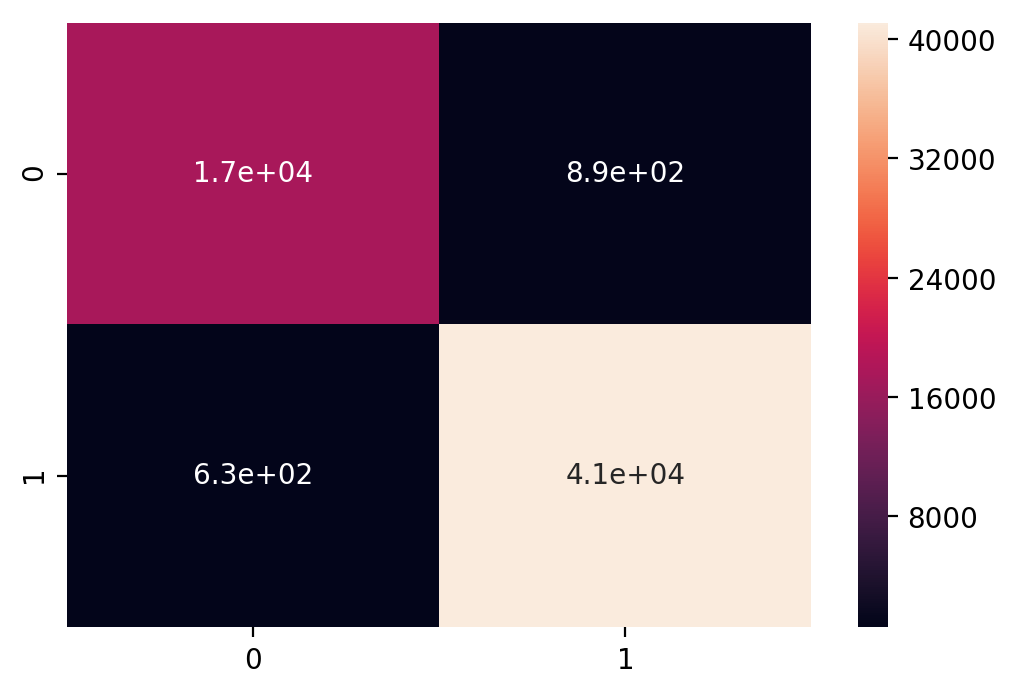
\includegraphics[width=0.32\textwidth]{./FigNSclass/CM_indRecCross}
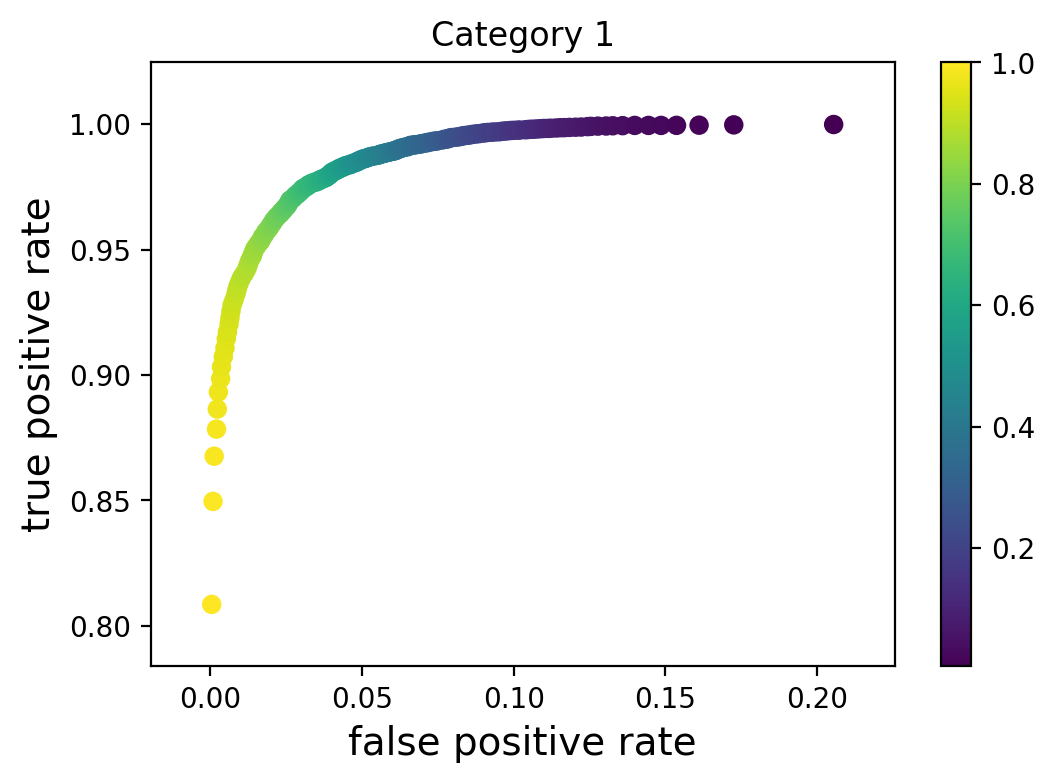
\includegraphics[width=0.32\textwidth]{./FigNSclass/rocCurve_indRecCross}
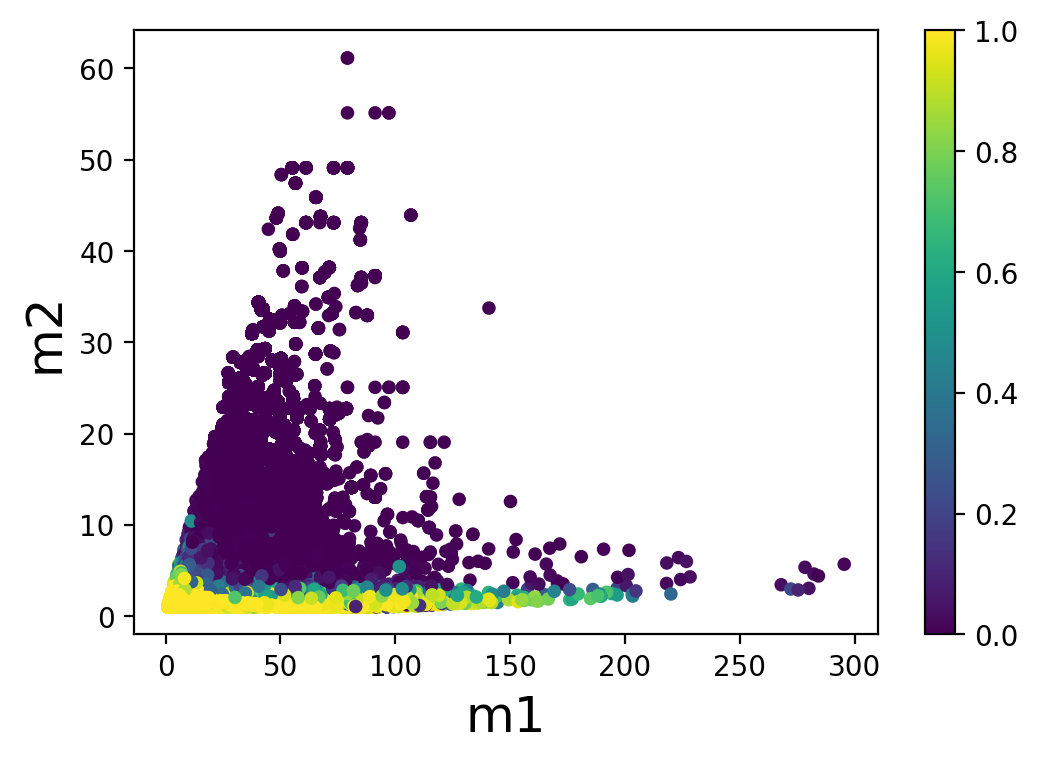
\includegraphics[width=0.32\textwidth]{./FigNSclass/scatterplot_indRecCross}
\caption{\label{fig:indreccross} Results with optimum model after crossvalidation. Using just independent recovered values (masses, spins and SNR).}
\end{figure}

\subsection{Using recovered variables}
Training and testing using: $m1_{rec}, m2_{rec}, chi1_{rec}, chi2_{rec}, mc_{rec}, q_{rec}, R_isco_{rec}, Compactness_{rec}, snr$.
Standard deviation of score during crossvalidation:  0.0002807499052054315 . Mean:  0.9744466574442907
Score  0.975032917215287 . Optimum forest found:  400  trees,  entropy  criteria and  sqrt  max features

Score on testing:  0.9745329088818147


\begin{figure}[]
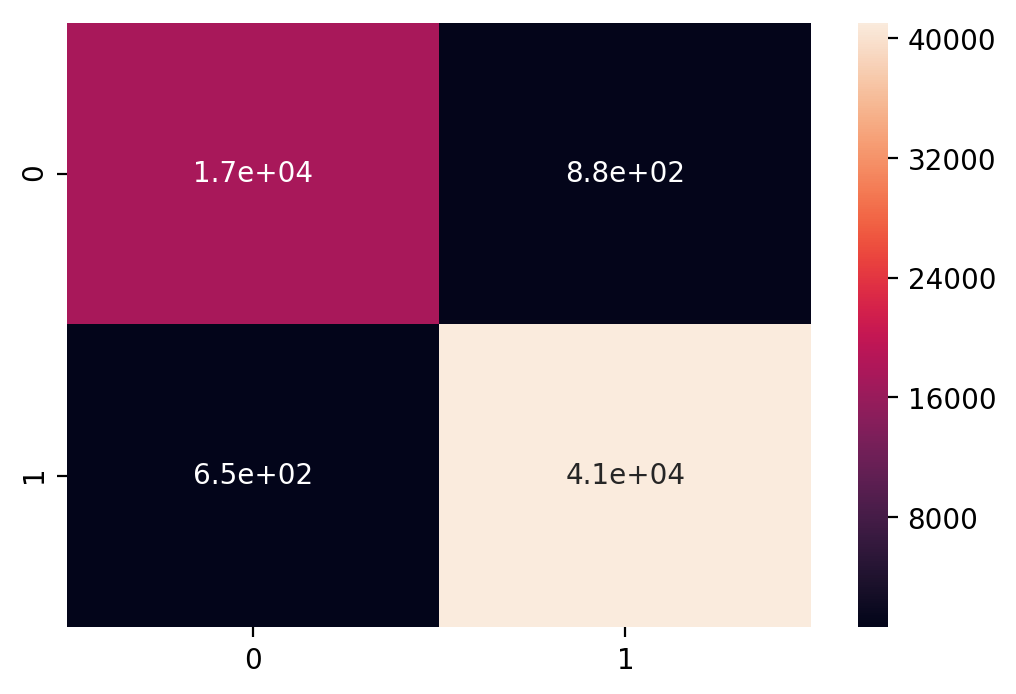
\includegraphics[width=0.32\textwidth]{./FigNSclass/CM_RecCross}
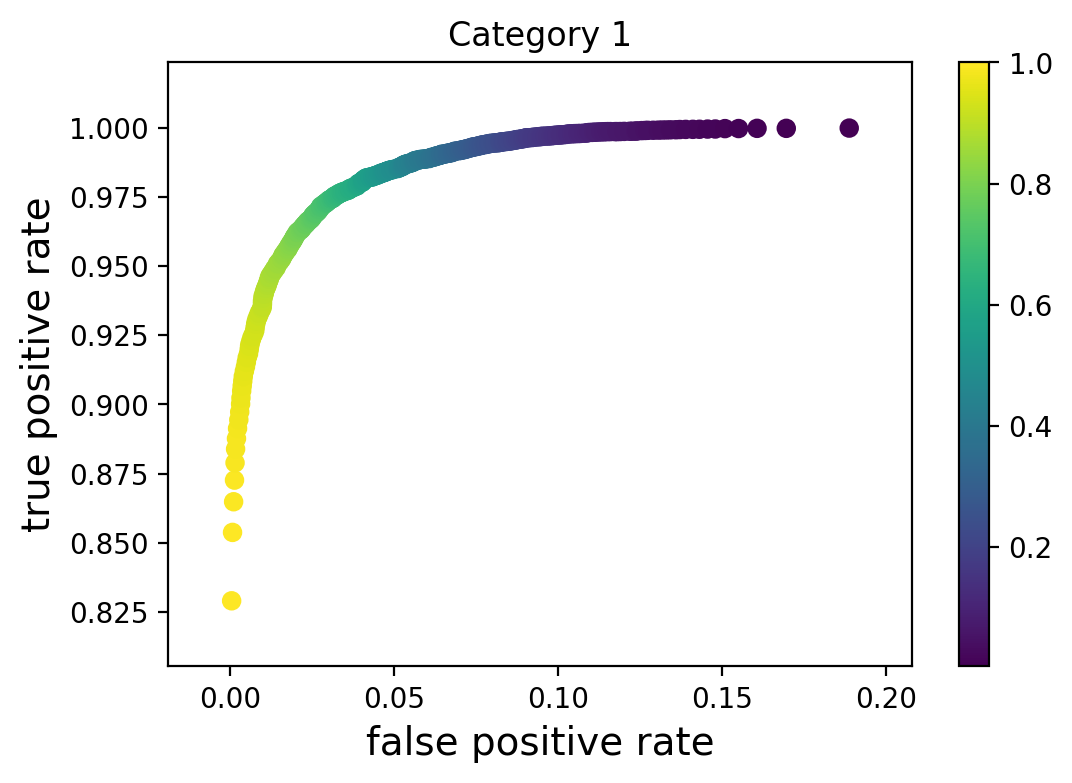
\includegraphics[width=0.32\textwidth]{./FigNSclass/rocCurve_RecCross}
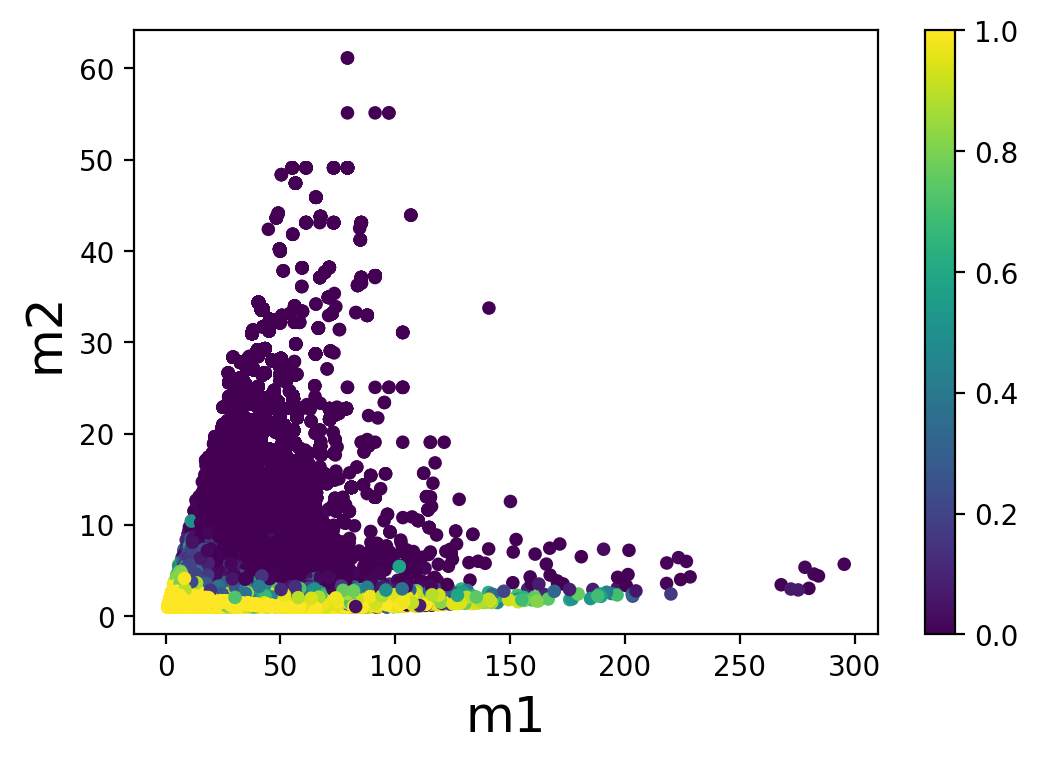
\includegraphics[width=0.32\textwidth]{./FigNSclass/scatterplot_RecCross}
\caption{\label{fig:indreccross} Results with optimum model after crossvalidation. Using all recovered values (masses, spins and SNR, mass ratio, chirp mass, compactness and Risco).}
\end{figure}

\subsection{All injected values}
No crossvalidated
Score on testing:  0.9999833330555509

\begin{figure}[]
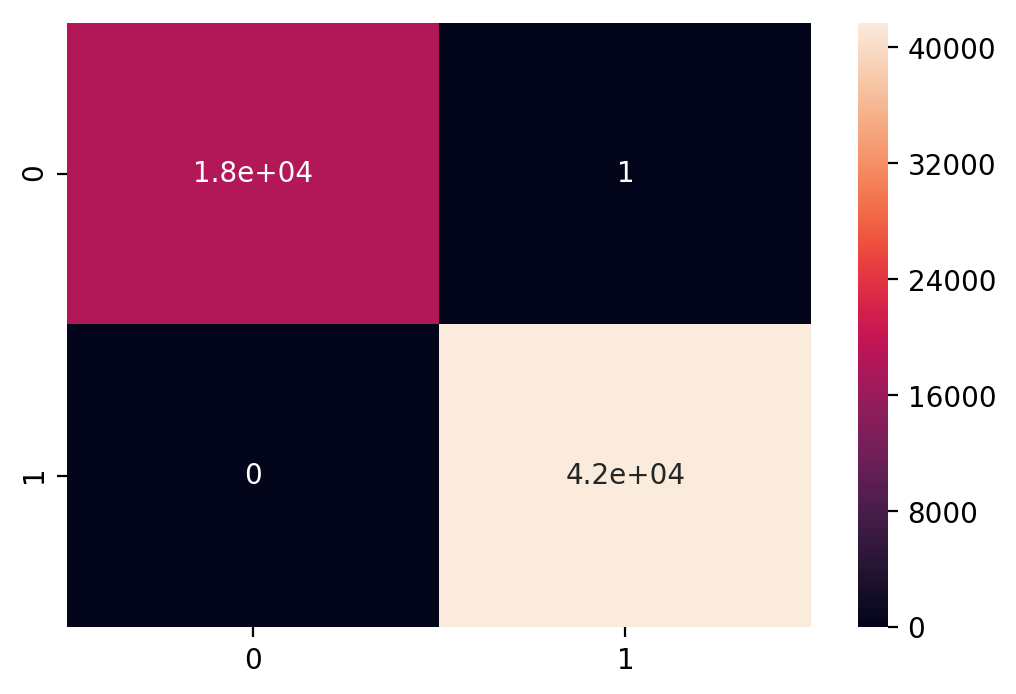
\includegraphics[width=0.32\textwidth]{./FigNSclass/CM_inj}
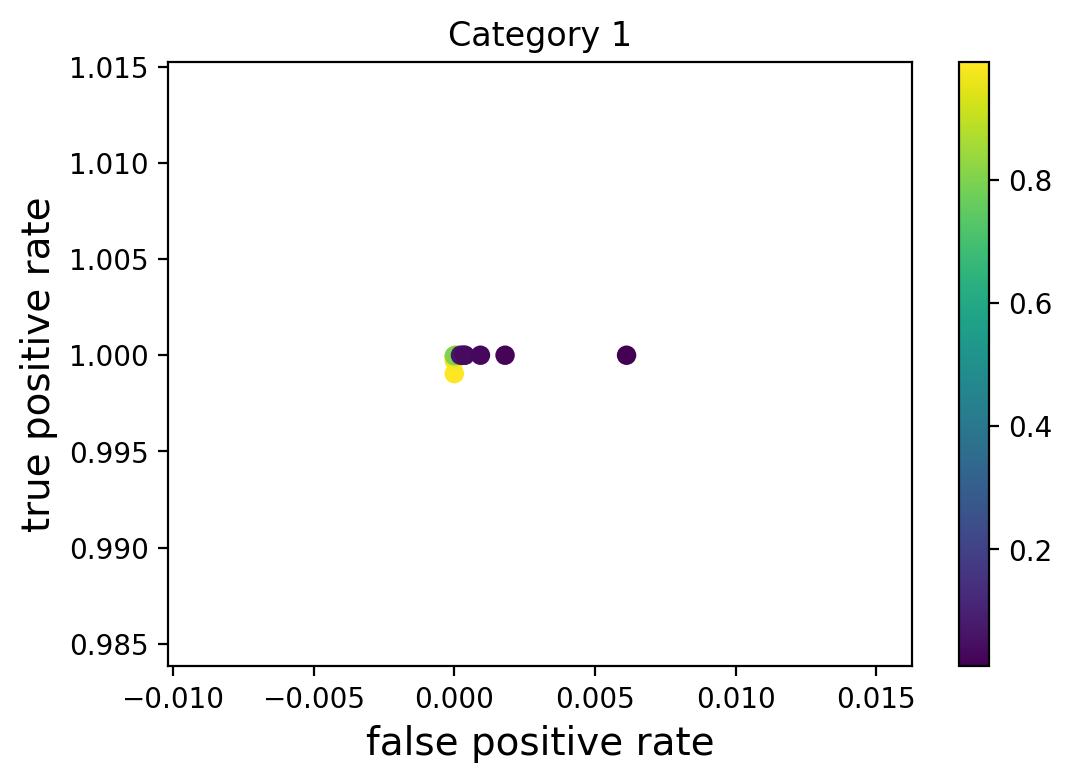
\includegraphics[width=0.32\textwidth]{./FigNSclass/rocCurve_inj}
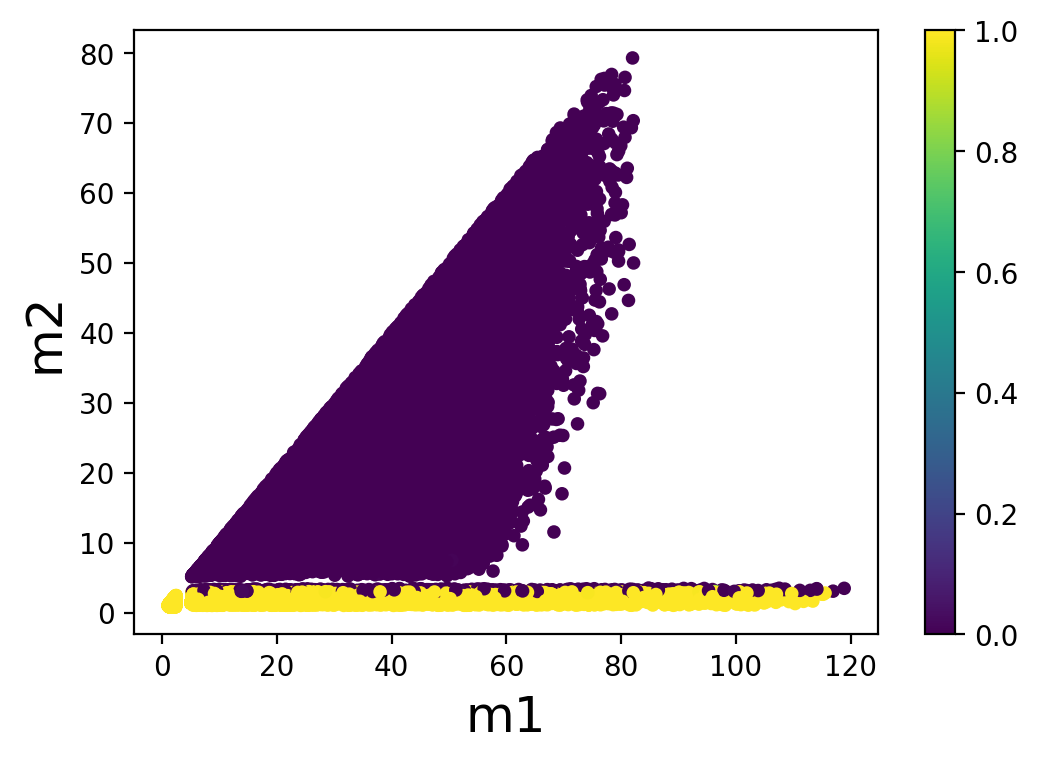
\includegraphics[width=0.32\textwidth]{./FigNSclass/scatterplot_inj}
\caption{\label{fig:inj} Results using all the injected values }
\end{figure}

\subsection{Independent injected values}
Score on testing:  0.9999833330555509

\begin{figure}[]
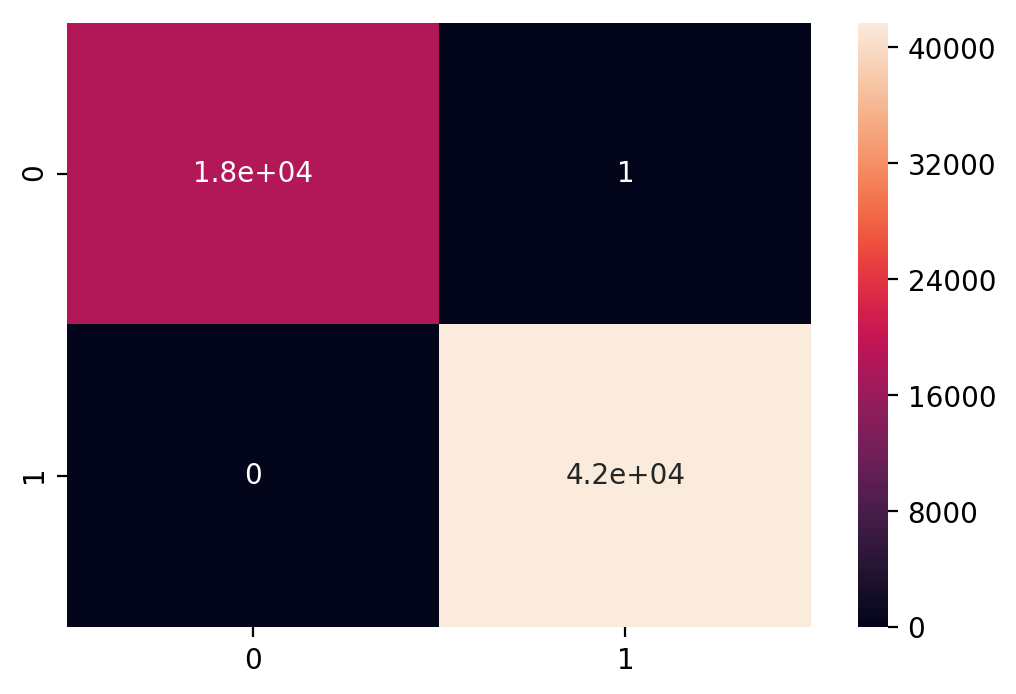
\includegraphics[width=0.32\textwidth]{./FigNSclass/CM_ind_inj}
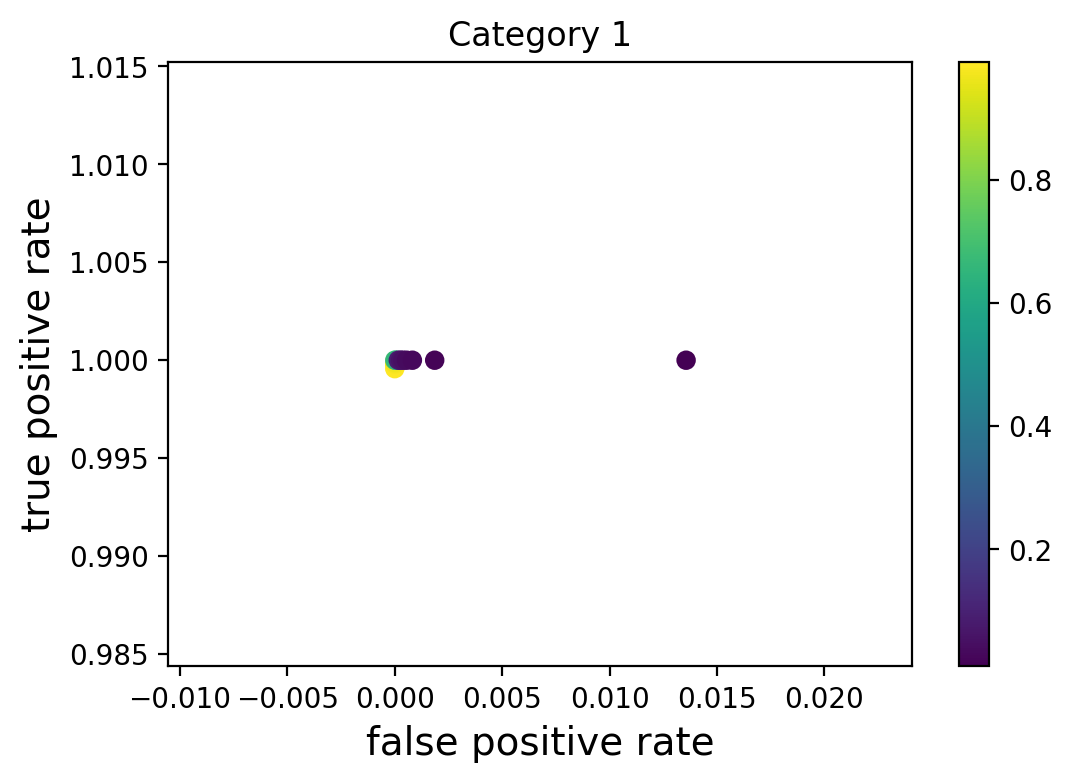
\includegraphics[width=0.32\textwidth]{./FigNSclass/rocCurve_ind_inj}
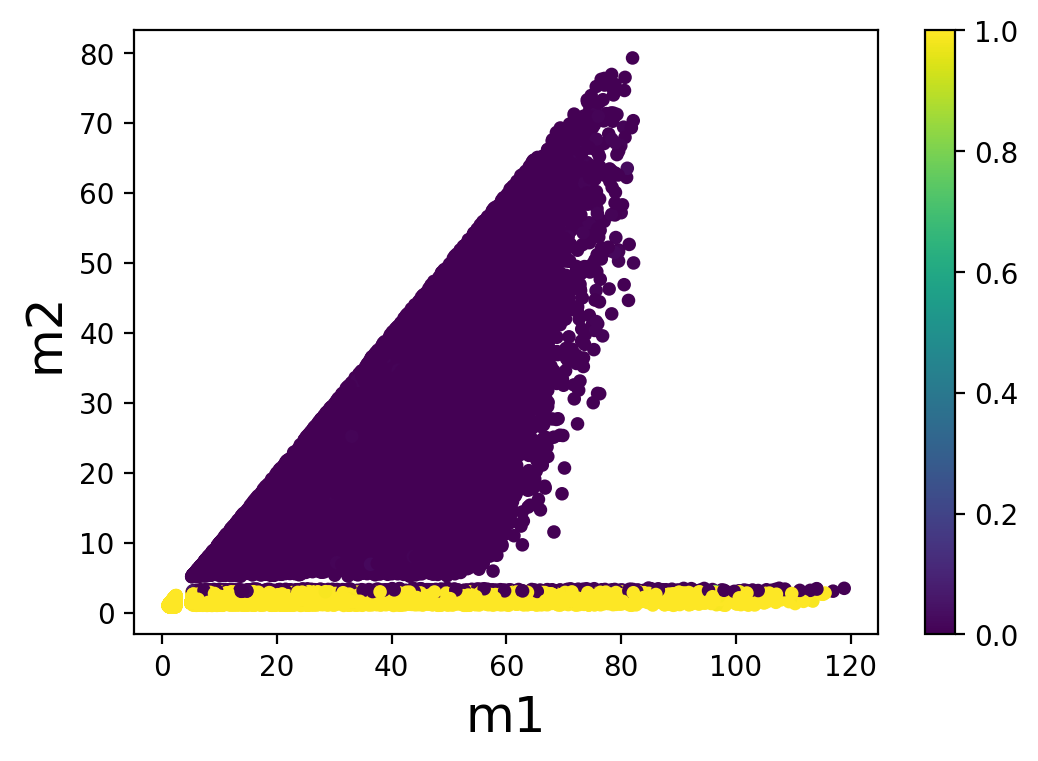
\includegraphics[width=0.32\textwidth]{./FigNSclass/scatterplot_ind_inj}
\caption{\label{fig:indinj} Results using the independent injected values}
\end{figure}

\newpage

%==========================================================
\section{K-Nearest Neighbors}
%==========================================================

In order to compare with Chatterjee et al (2020), we are only using 5 features, the independent variables: 
\begin{equation*}
	\big[m_1,m_2,\chi_1,\chi_2, \rm{SNR}\big]\,.
\end{equation*}
The study is made over the recovered values from GstLAL.  The mean score is computed by training the algorithm on the $90\%$ of the dataset and testing it on the remaining $10\%$, cycling the train/test combination over the full dataset. To do that, we are going to use the training dataset, sicne it's the larger one. In order to train and test the model and create the different plots, we are going to use the training and testing files. First of all, let's check the performance of the algorithm using the same parameters as in Chatterjee et al.

\subsection{Using paper's hyperparameters}
In this case, the number of neighbors is fixed to be $K=11$ (twice the number of features plus one). The metric usd is the Mahalanobis metric, but it is said that the metric used doesn't make too much difference. Points are weighted by the inverse of their distance.  The mean score is:
\begin{equation*}
	\rm{s_m} = 0.9668068999826518\,,
\end{equation*}
and the score on testing:
\begin{equation*}
	\rm{s_t} = 0.9673161219353655 \,.
\end{equation*}

The confusion matrix can be seen in Fig.~\ref{fig:confmatChat}. We have also plotted the $m_1$-$m_2$ plot with the probability of having a remnant, in Fig.~\ref{fig:m1m2Chat}, also with $q$ and $m_1$ in Fig.~\ref{fig:m1qChat}, and the true vs false positive rates with the corresponding threshold value for the probability in Fig.~\ref{fig:rocChat}.

\begin{figure}[]
    \includegraphics[width = 0.45\textwidth]{/Users/miquelmiravet/Projects/IPAM_LA/ML_group/KNN_miq/ipam_NS_set/plots_chatt/conf_matrix.pdf}
    \caption{Confusion matrix for the model used in Chatterjee et al (2020), using the independent recovered values. }
    \label{fig:confmatChat}
    \includegraphics[width = 0.4\textwidth]{/Users/miquelmiravet/Projects/IPAM_LA/ML_group/KNN_miq/ipam_NS_set/plots_chatt/m1m2prob.pdf}
    \caption{Probability of having a remnant as a function of the values of the masses.}
    \label{fig:m1m2Chat}
\end{figure}
\begin{figure}[]
    \includegraphics[width = 0.4\textwidth]{/Users/miquelmiravet/Projects/IPAM_LA/ML_group/KNN_miq/ipam_NS_set/plots_chatt/m1qprob.pdf}
    \caption{Probability of having a remnant as a function of $m_1$ and the mass ratio of the binary, $q$.}
    \label{fig:m1qChat}
    \includegraphics[width =0.4\textwidth]{/Users/miquelmiravet/Projects/IPAM_LA/ML_group/KNN_miq/ipam_NS_set/plots_chatt/ROCplot.pdf}
    \caption{Relation of the true and false positive rates as a function of the threshold applied to make the decision betweenhaving or not having a remnant. }
    \label{fig:rocChat}
\end{figure}

\newpage

\subsection{Using our hyperparameters}
In our case, the metric used to compute the distance between points is the \textit{Manhattan} metric, weighting the points uniformly. After applying cross validation, we get that the  optimal number of neighbors is $K = 10$, with a mean score of: 
\begin{equation*}
	\rm{s_m} = 0.9718355224352762\,,
\end{equation*}
and the score of testing
\begin{equation*}
	\rm{s_t} = 0.9723828730478842\,.
\end{equation*}

\begin{figure}[]
    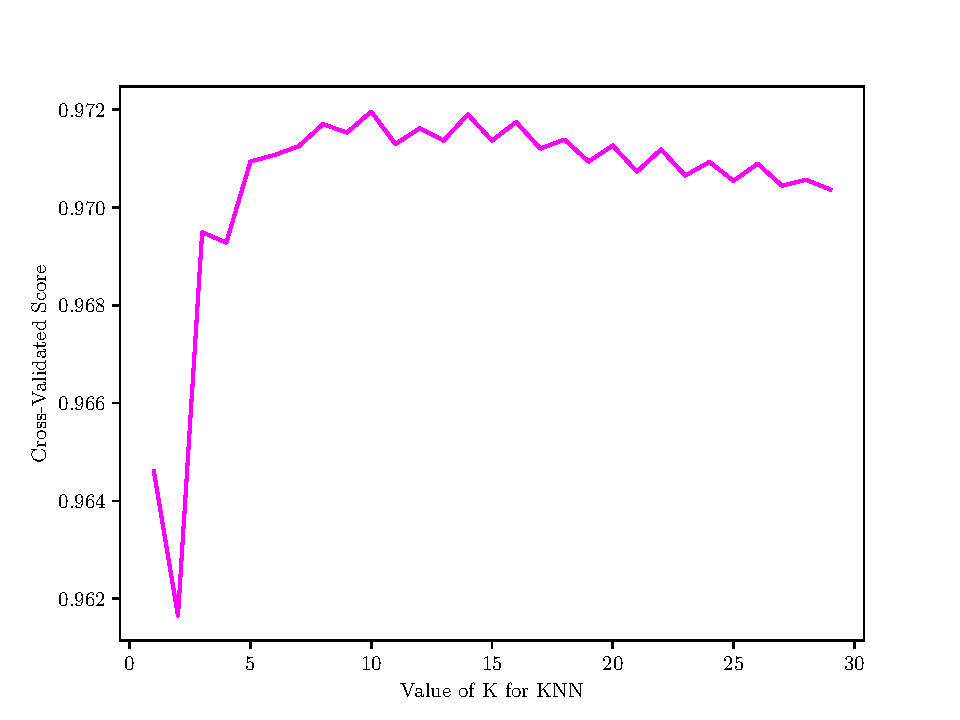
\includegraphics[width = 0.4\textwidth]{/Users/miquelmiravet/Projects/IPAM_LA/ML_group/KNN_miq/ipam_NS_set/plots_miq/CrossValK.pdf}
    \caption{Score of our model as a function of the number of neighbors.}
    \label{fig:crossvalK}
    \end{figure}

In Fig.~\ref{fig:crossvalK} you can find how the mean score changes with the number of neighbors of the algorithm.  The confusion matrix appears in Fig.~\ref{fig:confmat}, the probability as a function of $m_1$ and $m_2$ and $m_1$ and q is shown in Figs.~\ref{fig:m1m2},~\ref{fig:m1q}, respectively, and the true and false positive rates in terms of the threshold probability appear in Fig.~\ref{fig:roc}.

\begin{figure}[]
    \includegraphics[width = 0.45\textwidth]{/Users/miquelmiravet/Projects/IPAM_LA/ML_group/KNN_miq/ipam_NS_set/plots_miq/conf_matrix.pdf}
    \caption{Confusion matrix for our model, using the independent recovered values. }
    \label{fig:confmat}
    \includegraphics[width = 0.4\textwidth]{/Users/miquelmiravet/Projects/IPAM_LA/ML_group/KNN_miq/ipam_NS_set/plots_miq/m1m2prob.pdf}
    \caption{Probability of having a remnant as a function of the values of the masses.}
    \label{fig:m1m2}
\end{figure}
\begin{figure}[]
    \includegraphics[width = 0.4\textwidth]{/Users/miquelmiravet/Projects/IPAM_LA/ML_group/KNN_miq/ipam_NS_set/plots_miq/m1qprob.pdf}
    \caption{Probability of having a remnant as a function of $m_1$ and the mass ratio of the binary, $q$.}
    \label{fig:m1q}
    \includegraphics[width =0.4\textwidth]{/Users/miquelmiravet/Projects/IPAM_LA/ML_group/KNN_miq/ipam_NS_set/plots_miq/ROCplot.pdf}
    \caption{Relation of the true and false positive rates as a function of the threshold applied to make the decision between having or not having a remnant. }
    \label{fig:roc}
\end{figure}


\end{document}